% Options for packages loaded elsewhere
\PassOptionsToPackage{unicode}{hyperref}
\PassOptionsToPackage{hyphens}{url}
%
\documentclass[
]{scrartcl}
\usepackage{amsmath,amssymb}
\usepackage{lmodern}
\usepackage{iftex}
\ifPDFTeX
  \usepackage[T1]{fontenc}
  \usepackage[utf8]{inputenc}
  \usepackage{textcomp} % provide euro and other symbols
\else % if luatex or xetex
  \usepackage{unicode-math}
  \defaultfontfeatures{Scale=MatchLowercase}
  \defaultfontfeatures[\rmfamily]{Ligatures=TeX,Scale=1}
\fi
% Use upquote if available, for straight quotes in verbatim environments
\IfFileExists{upquote.sty}{\usepackage{upquote}}{}
\IfFileExists{microtype.sty}{% use microtype if available
  \usepackage[]{microtype}
  \UseMicrotypeSet[protrusion]{basicmath} % disable protrusion for tt fonts
}{}
\makeatletter
\@ifundefined{KOMAClassName}{% if non-KOMA class
  \IfFileExists{parskip.sty}{%
    \usepackage{parskip}
  }{% else
    \setlength{\parindent}{0pt}
    \setlength{\parskip}{6pt plus 2pt minus 1pt}}
}{% if KOMA class
  \KOMAoptions{parskip=half}}
\makeatother
\usepackage{xcolor}
\IfFileExists{xurl.sty}{\usepackage{xurl}}{} % add URL line breaks if available
\IfFileExists{bookmark.sty}{\usepackage{bookmark}}{\usepackage{hyperref}}
\hypersetup{
  pdftitle={Codebook bundeslaendeR},
  pdfauthor={Robert Stelzle},
  hidelinks,
  pdfcreator={LaTeX via pandoc}}
\urlstyle{same} % disable monospaced font for URLs
\usepackage[lmargin=2.5cm, rmargin=3.5cm, tmargin=2.5cm, bmargin=2.5cm,
includeheadfoot]{geometry}
\usepackage{color}
\usepackage{fancyvrb}
\newcommand{\VerbBar}{|}
\newcommand{\VERB}{\Verb[commandchars=\\\{\}]}
\DefineVerbatimEnvironment{Highlighting}{Verbatim}{commandchars=\\\{\}}
% Add ',fontsize=\small' for more characters per line
\usepackage{framed}
\definecolor{shadecolor}{RGB}{248,248,248}
\newenvironment{Shaded}{\begin{snugshade}}{\end{snugshade}}
\newcommand{\AlertTok}[1]{\textcolor[rgb]{0.94,0.16,0.16}{#1}}
\newcommand{\AnnotationTok}[1]{\textcolor[rgb]{0.56,0.35,0.01}{\textbf{\textit{#1}}}}
\newcommand{\AttributeTok}[1]{\textcolor[rgb]{0.77,0.63,0.00}{#1}}
\newcommand{\BaseNTok}[1]{\textcolor[rgb]{0.00,0.00,0.81}{#1}}
\newcommand{\BuiltInTok}[1]{#1}
\newcommand{\CharTok}[1]{\textcolor[rgb]{0.31,0.60,0.02}{#1}}
\newcommand{\CommentTok}[1]{\textcolor[rgb]{0.56,0.35,0.01}{\textit{#1}}}
\newcommand{\CommentVarTok}[1]{\textcolor[rgb]{0.56,0.35,0.01}{\textbf{\textit{#1}}}}
\newcommand{\ConstantTok}[1]{\textcolor[rgb]{0.00,0.00,0.00}{#1}}
\newcommand{\ControlFlowTok}[1]{\textcolor[rgb]{0.13,0.29,0.53}{\textbf{#1}}}
\newcommand{\DataTypeTok}[1]{\textcolor[rgb]{0.13,0.29,0.53}{#1}}
\newcommand{\DecValTok}[1]{\textcolor[rgb]{0.00,0.00,0.81}{#1}}
\newcommand{\DocumentationTok}[1]{\textcolor[rgb]{0.56,0.35,0.01}{\textbf{\textit{#1}}}}
\newcommand{\ErrorTok}[1]{\textcolor[rgb]{0.64,0.00,0.00}{\textbf{#1}}}
\newcommand{\ExtensionTok}[1]{#1}
\newcommand{\FloatTok}[1]{\textcolor[rgb]{0.00,0.00,0.81}{#1}}
\newcommand{\FunctionTok}[1]{\textcolor[rgb]{0.00,0.00,0.00}{#1}}
\newcommand{\ImportTok}[1]{#1}
\newcommand{\InformationTok}[1]{\textcolor[rgb]{0.56,0.35,0.01}{\textbf{\textit{#1}}}}
\newcommand{\KeywordTok}[1]{\textcolor[rgb]{0.13,0.29,0.53}{\textbf{#1}}}
\newcommand{\NormalTok}[1]{#1}
\newcommand{\OperatorTok}[1]{\textcolor[rgb]{0.81,0.36,0.00}{\textbf{#1}}}
\newcommand{\OtherTok}[1]{\textcolor[rgb]{0.56,0.35,0.01}{#1}}
\newcommand{\PreprocessorTok}[1]{\textcolor[rgb]{0.56,0.35,0.01}{\textit{#1}}}
\newcommand{\RegionMarkerTok}[1]{#1}
\newcommand{\SpecialCharTok}[1]{\textcolor[rgb]{0.00,0.00,0.00}{#1}}
\newcommand{\SpecialStringTok}[1]{\textcolor[rgb]{0.31,0.60,0.02}{#1}}
\newcommand{\StringTok}[1]{\textcolor[rgb]{0.31,0.60,0.02}{#1}}
\newcommand{\VariableTok}[1]{\textcolor[rgb]{0.00,0.00,0.00}{#1}}
\newcommand{\VerbatimStringTok}[1]{\textcolor[rgb]{0.31,0.60,0.02}{#1}}
\newcommand{\WarningTok}[1]{\textcolor[rgb]{0.56,0.35,0.01}{\textbf{\textit{#1}}}}
\usepackage{graphicx}
\makeatletter
\def\maxwidth{\ifdim\Gin@nat@width>\linewidth\linewidth\else\Gin@nat@width\fi}
\def\maxheight{\ifdim\Gin@nat@height>\textheight\textheight\else\Gin@nat@height\fi}
\makeatother
% Scale images if necessary, so that they will not overflow the page
% margins by default, and it is still possible to overwrite the defaults
% using explicit options in \includegraphics[width, height, ...]{}
\setkeys{Gin}{width=\maxwidth,height=\maxheight,keepaspectratio}
% Set default figure placement to htbp
\makeatletter
\def\fps@figure{htbp}
\makeatother
\setlength{\emergencystretch}{3em} % prevent overfull lines
\providecommand{\tightlist}{%
  \setlength{\itemsep}{0pt}\setlength{\parskip}{0pt}}
\setcounter{secnumdepth}{-\maxdimen} % remove section numbering
\usepackage{longtable}
\usepackage{float}
\usepackage{graphicx}
\usepackage{pdflscape}
\newcommand{\blandscape}{\begin{landscape}}
\newcommand{\elandscape}{\end{landscape}}
\usepackage{fontspec}
\usepackage{libertinus}
\usepackage{enumitem}
\setmonofont[Scale=MatchLowercase,FakeStretch=0.9]{Consolas}
\setkomafont{captionlabel}{\bfseries\small\sffamily}
\setkomafont{caption}{\small\sffamily}
\usepackage[automark, headsepline=1pt, footsepline=1pt]{scrlayer-scrpage}
\ohead{Codebook bundeslaendeR}
\ofoot*{20.08.2022} \ihead{\headmark}
\setkomafont{pagenumber}{\itshape}
\ifoot*{Seite \pagemark}
\chead{}
\cfoot*{}
\usepackage{titling}
\pretitle{\begin{center} 
\includegraphics[width=2in,height=2in]{../man/figures/hex_light_clipart.png}\LARGE\\}
\posttitle{\end{center}}
\usepackage{booktabs}
\usepackage{longtable}
\usepackage{array}
\usepackage{multirow}
\usepackage{wrapfig}
\usepackage{float}
\usepackage{colortbl}
\usepackage{pdflscape}
\usepackage{tabu}
\usepackage{threeparttable}
\usepackage{threeparttablex}
\usepackage[normalem]{ulem}
\usepackage{makecell}
\usepackage{xcolor}
\ifLuaTeX
  \usepackage{selnolig}  % disable illegal ligatures
\fi
\usepackage[backref,style=ext-authoryear-comp,minnames=1,maxnames=3,isbn=false,date=year,sorting=nyt]{biblatex}
\addbibresource{literature.bib}

\title{Codebook bundeslaendeR}
\author{Robert Stelzle}
\date{20.08.2022}

\begin{document}
\maketitle

{
\setcounter{tocdepth}{1}
\tableofcontents
}
\clearpage

\hypertarget{introduction}{%
\section{Introduction}\label{introduction}}

Most election results data are provided by the Bundeswahlleiter. A
machine-readable version of the Bundeswahlleiter's compiled data
contained in the -periodically published- pdf available here
(\url{https://www.bundeswahlleiter.de/service/landtagswahlen.html}) was
kindly provided to me. Election data outside the timeframe covered by
Bundeswahlleiter's data provided to me was collected from the states'
local election authorities' (Landeswahlleiter) websites. More
information on parties and the continuity of parties under different
labels was collected by me.

The Bundeswahlleiter's election data in many cases contains differing
names for the same party. Both between states (eg. ``Christlich
Demokratische Union Deutschlands'' vs.~``Christlich Demokratische Union
Deutschlands in Niedersachsen'') as well as within states between
elections -in many cases due to parties being renamed- (``BÜNDNIS 90/DIE
GRÜNEN, Landesverband Hamburg, Grün-Alternative Liste'' vs.~``BÜNDNIS
90/DIE GRÜNEN, Landesverband Hamburg''). Efforts were made to reconcile
both of these inconsistencies by adding two new, harmonized variables
identifying parties (\texttt{partyname\_short} and \texttt{partyname}).
This harmonized party identifier also covers merging of parties. The
partyname given to the resulting party (eg. ``Linke'', ``Grüne'') is
given to the largest of the preceding parties contesting an election
unless a smaller party joined a government following the election. The
original names provided by the Bundeswahlleiter (and Landeswahlleiters
in elections after June 2021) are still available
(\texttt{partyname\_short\_bundeswahlleiter} and
\texttt{partyname\_bundeswahlleiter}).

Information on governments is mainly taken from replication data from
\textcite{linhartProportionaleMinisterienaufteilungDeutschen2008} which
can be found online here:
\url{https://www.tu-chemnitz.de/phil/politik/pspi/forschung/daten.php}.
Information outside the timeframe of Linhart et al.~as well as
information on the names and party affiliations of the
Ministerpräsidenten was collected by me, mainly from German Wikipedia.

All datasets can be accessed through the \texttt{R} Package
\texttt{bundeslaendeR}.
\footnote{Calling \texttt{bundeslaender::ltw\_elections}, \texttt{bundeslaender::ltw\_governments} , \texttt{bundeslaender::ltw\_combined},
\texttt{bundeslaender::ltw\_elections\_meta}, \texttt{bundeslaender::link\_manifestos} and \texttt{bundeslaender::link\_coalitionagreements}.}
This package further includes one function
-\texttt{bundeslaendeR::de\_states\_geofacet\_grid\_4x4()}- that is
documented below. Alternatively all datasets can be downloaded in a
single \texttt{.zip} file including all six datasets as \texttt{.csv},
\texttt{.rds} and \texttt{.dta} files.

\newpage

\hypertarget{ltw_elections}{%
\section{\texorpdfstring{\texttt{ltw\_elections}}{ltw\_elections}}\label{ltw_elections}}

\texttt{ltw\_elections} is a long-form dataset containing one row per
contesting party per election. For a schematic version of
\texttt{ltw\_elections}'s structure see table\(~\)\ref{strltwelecres}.
The data can be accessed in \texttt{R} using
\texttt{bundeslaendeR::ltw\_elections}.

\begin{table}
\centering
\caption{Structure of \texttt{ltw\_elections}}
\label{strltwelecres}
\tiny
\texttt{
\begin{tabular}{llrllrllrllr}
            \toprule
            \multicolumn{3}{c}{\textbf{\textsf{State Variables}}} & \multicolumn{3}{c}{\textbf{\textsf{Election Variables}}} & \multicolumn{3}{c}{\textbf{\textsf{Party Variables}}} & \multicolumn{3}{c}{\textbf{\textsf{Party-Election Variables}}}\\
            \multicolumn{3}{c}{\textsf{Name, Abbreviation, NUTS1 Code}} & \multicolumn{3}{c}{\textsf{Election date, Size Electorate, Turnout, ...}} & \multicolumn{3}{c}{\textsf{Names, Abbreviations, several IDs}} & \multicolumn{3}{c}{\textsf{Vote Count, -Share, Seat Count, -Share, ...}}\\
            \cmidrule(r){1-3}\cmidrule(lr){4-6}\cmidrule(lr){7-9}\cmidrule(l){10-12}
            \textbf{state} & \textbf{nuts1} & \textbf{...} & \textbf{election\_date} & \textbf{turnout} & \textbf{...} & \textbf{partyname\_short} & \textbf{ches\_id} & \textbf{...} & \textbf{party\_vshare} & \textbf{party\_seat\_count} & \textbf{...} \\
            \midrule
            BE & DE3 & ... & 2015-09-18 & 0.765 & ... & Party A & 001 & ... & 0.45 & 46 & ...\\
            BE & DE3 & ... & 2015-09-18 & 0.765 & ... & Party B & 002 & ... & 0.30 & 12 & ...\\
            BE & DE3 & ... & 2015-09-18 & 0.765 & ... & Party C & 003 & ... & 0.25 & 18 & ...\\
        &&&&&&&&&&&\\[-2ex]
            NI & DE9 & ... & 2012-12-16 & 0.560 & ... & Party A & 001 & ... & 0.17 & 12 & ...\\
            NI & DE9 & ... & 2012-12-16 & 0.560 & ... & Party B & 002 & ... & 0.33 & 27 & ...\\
            NI & DE9 & ... & 2012-12-16 & 0.560 & ... & Party D & 004 & ... & 0.50 & 46 & ...\\
            \bottomrule
    \end{tabular}}


\end{table}

\hypertarget{ltw_elections-variable-information}{%
\subsection{\texorpdfstring{\texttt{ltw\_elections} Variable
Information}{ltw\_elections Variable Information}}\label{ltw_elections-variable-information}}

\begin{longtable}{p{3.2cm}| p{11cm}}
\texttt{state} &\textbf{State Abbreviation}\newline 
ISO 3166-2:DE-code of the state;
           including BA for the former state of Baden, WH for the former state
           of Württemberg-Hohenzollern and WB for the former state of
           Württemberg-Baden.
\end{longtable}

\begin{longtable}{p{3.2cm}| p{11cm}}
\texttt{nuts1} &\textbf{NUTS1 Code of State}\newline 
NUTS1 code of state. NA for former states Baden, Württemberg-Baden, Württemberg-Hohenzollern.
\end{longtable}

\begin{longtable}{p{3.2cm}| p{11cm}}
\texttt{state\_name\_de} &\textbf{German Name of State}\newline 
German name of the state.
\end{longtable}

\begin{longtable}{p{3.2cm}| p{11cm}}
\texttt{state\_name\_en} &\textbf{English Name of State.}\newline 
English name of the state.
\end{longtable}

\begin{longtable}{p{3.2cm}| p{11cm}}
\texttt{state\_election\_
term} &\textbf{Election Term of State}\newline 
Election term in the state. Counts up from 1.



\hspace*{.25cm}
\begin{minipage}[t]{\linewidth }
\vspace{0pt}
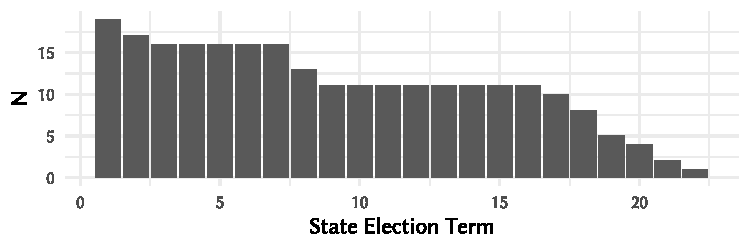
\includegraphics[width = \linewidth]{cbfiles/electiontermplot.pdf}
\end{minipage}



\end{longtable}

\begin{longtable}{p{3.2cm}| p{11cm}}
\texttt{election\_date} &\textbf{Election Date}\newline 
Date of the election.  ISO 8601 or R-Date format.






\hspace*{.25cm}
\begin{minipage}[t]{\linewidth }
\vspace{0pt}
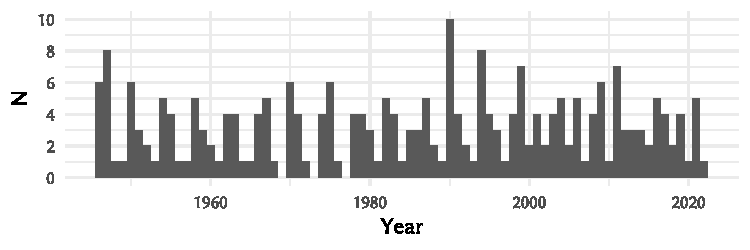
\includegraphics[width = \linewidth]{cbfiles/electiondatesplot.pdf}
\end{minipage}






\end{longtable}

\begin{longtable}{p{3.2cm}| p{11cm}}
\texttt{election\_id\_
bundeswahlleiter} &\textbf{Election ID Bundeswahlleiter}\newline 
Specific election\_id as denoted by the Bundeswahlleiter. Note that BA, WH and WH are named as BW and the number counts down. NA for cases taken from Landeswahlleiters (i.e. elections after ST 2021).
\end{longtable}

\begin{longtable}{p{3.2cm}| p{11cm}}
\texttt{election\_remarks\_
wahlleiter} &\textbf{Election Remarks Bundeswahlleiter}\newline 
Remarks on the election as given by the Bundeswahlleiter.
\end{longtable}

\begin{longtable}{p{3.2cm}| p{11cm}}
\texttt{electorate} &\textbf{Size of the Electorate}\newline 
Number of eligible voters. For more totals also see the last six columns.

\hspace*{.25cm}
\begin{minipage}[t]{\linewidth }
\vspace{0pt}
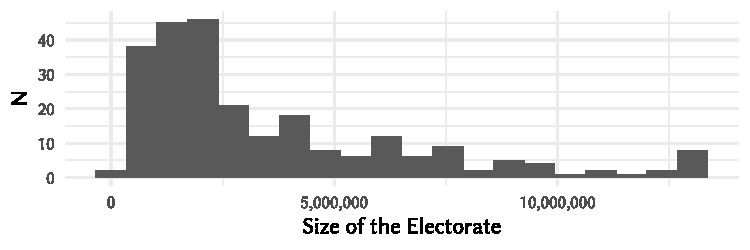
\includegraphics[width = \linewidth]{cbfiles/electorateplot.pdf}
\end{minipage}


\end{longtable}

\begin{longtable}{p{3.2cm}| p{11cm}}
\texttt{number\_of\_voters} &\textbf{Number of Voters}\newline 
Number of voters turning out. For more totals also see the last six columns.

\hspace*{.25cm}
\begin{minipage}[t]{\linewidth }
\vspace{0pt}
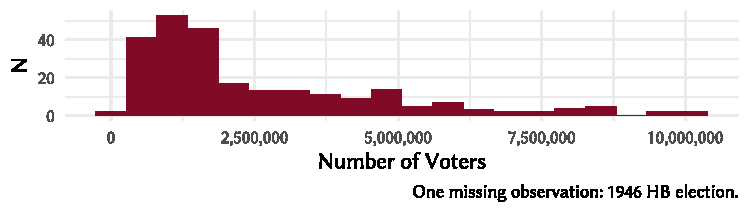
\includegraphics[width = \linewidth]{cbfiles/nvotersplot.pdf}
\end{minipage}


\end{longtable}

\begin{longtable}{p{3.2cm}| p{11cm}}
\texttt{turnout} &\textbf{Turnout}\newline 
Turnout. Share of eligible voters turning out.

\hspace*{.25cm}
\begin{minipage}[t]{\linewidth }
\vspace{0pt}
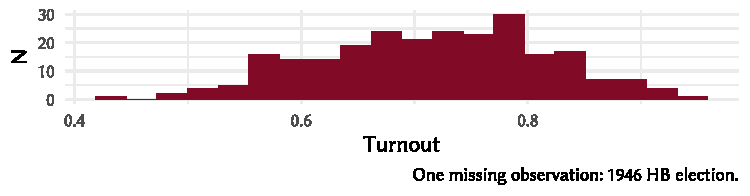
\includegraphics[width = \linewidth]{cbfiles/turnoutplot.pdf}
\end{minipage}


\end{longtable}

\begin{longtable}{p{3.2cm}| p{11cm}}
\texttt{valid\_votes} &\textbf{Valid Votes}\newline 
Number of valid votes. Does not have to be equal to the number of ballots cast, as sometimes a ballot contains multiple votes! For more totals also see the last six columns.

\hspace*{.25cm}
\begin{minipage}[t]{\linewidth }
\vspace{0pt}
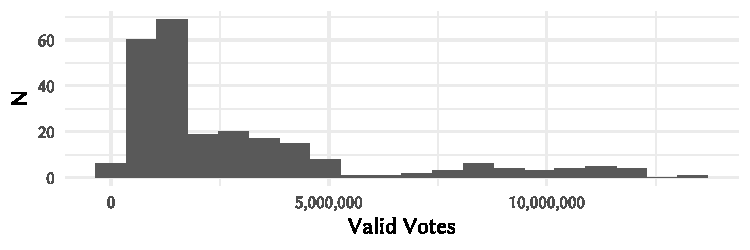
\includegraphics[width = \linewidth]{cbfiles/validvoteplot.pdf}
\end{minipage}


\end{longtable}

\begin{longtable}{p{3.2cm}| p{11cm}}
\texttt{total\_seats\_
parliament} &\textbf{Total Seats in Parliament}\newline 
Total number of members of the newly elected Landtag.

\hspace*{.25cm}
\begin{minipage}[t]{\linewidth }
\vspace{0pt}
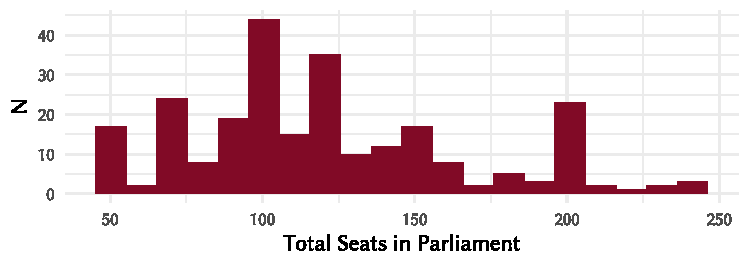
\includegraphics[width = \linewidth]{cbfiles/tseatsparlplot.pdf}
\end{minipage}


\end{longtable}

\begin{longtable}{p{3.2cm}| p{11cm}}
\texttt{female\_party\_
seats\_available} &\textbf{Number of female MdLs available per party}\newline 
Denotes whether information on the no. of female members of the Landtag per party is available for this election. Note that for parties not elected to the new Landtag party\_female\_mps always is marked as missing.

\hspace*{.25cm}
\begin{minipage}[t]{\linewidth }
\vspace{0pt}
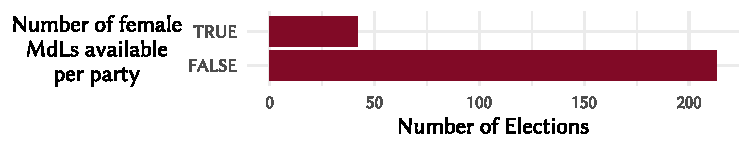
\includegraphics[width = \linewidth]{cbfiles/fpsaplot.pdf}
\end{minipage}


\end{longtable}

\begin{longtable}{p{3.2cm}| p{11cm}}
\texttt{total\_female\_
mps\_parliament} &\textbf{Number of Female MPs in Parliament}\newline 
Number of newly elected female MPs.

\hspace*{.25cm}
\begin{minipage}[t]{\linewidth }
\vspace{0pt}
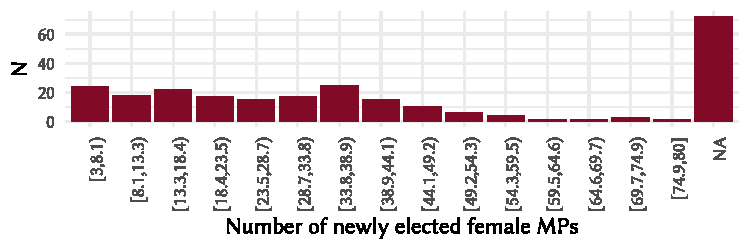
\includegraphics[width = \linewidth]{cbfiles/totfemmpsplot.pdf}
\end{minipage}


\end{longtable}

\begin{longtable}{p{3.2cm}| p{11cm}}
\texttt{partyname\_short} &\textbf{Abbreviated Party Name}\newline 
Harmonized abbreviation of the party's name. 379 unique parties.
\end{longtable}

\begin{longtable}{p{3.2cm}| p{11cm}}
\texttt{partyname} &\textbf{Party Name}\newline 
Harmonized name of the party. 379 unique parties.
\end{longtable}

\begin{longtable}{p{3.2cm}| p{11cm}}
\texttt{partyname\_short\_
bundeswahlleiter} &\textbf{Party Name Abbreviation from Bundeswahlleiter}\newline 
Partyname abbreviation as documented by the Bundeswahlleiter. 467 different abbreviations.
\end{longtable}

\begin{longtable}{p{3.2cm}| p{11cm}}
\texttt{partyname\_
bundeswahlleiter} &\textbf{Party Name from Bundeswahlleiter}\newline 
Partyname as documented by the Bundeswahlleiter. 508 different names.
\end{longtable}

\begin{longtable}{p{3.2cm}| p{11cm}}
\texttt{party\_vote\_count} &\textbf{Party Vote Count}\newline 
Number of votes recieved by the party.

\hspace*{.25cm}
\begin{minipage}[t]{\linewidth }
\vspace{0pt}
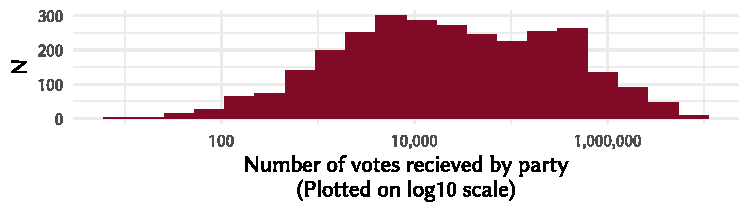
\includegraphics[width = \linewidth]{cbfiles/pvcplot.pdf}
\end{minipage}


\end{longtable}

\begin{longtable}{p{3.2cm}| p{11cm}}
\texttt{party\_vshare} &\textbf{Party Vote Share}\newline 
Share of votes recieved by the party.

\hspace*{.25cm}
\begin{minipage}[t]{\linewidth }
\vspace{0pt}
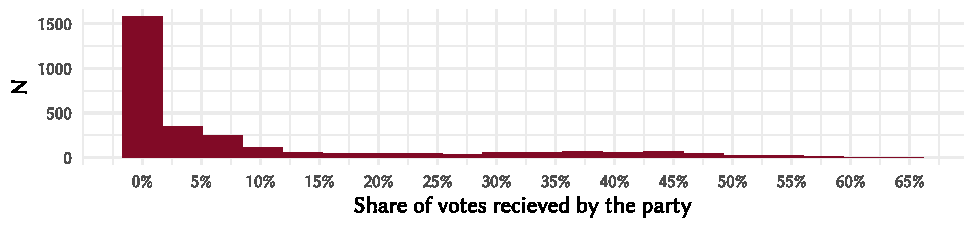
\includegraphics[width = \linewidth]{cbfiles/pvsplot.pdf}
\end{minipage}


\end{longtable}

\begin{longtable}{p{3.2cm}| p{11cm}}
\texttt{party\_seat\_count} &\textbf{Party Seat Count}\newline 
Number of seats recieved by the party.

\hspace*{.25cm}
\begin{minipage}[t]{\linewidth }
\vspace{0pt}
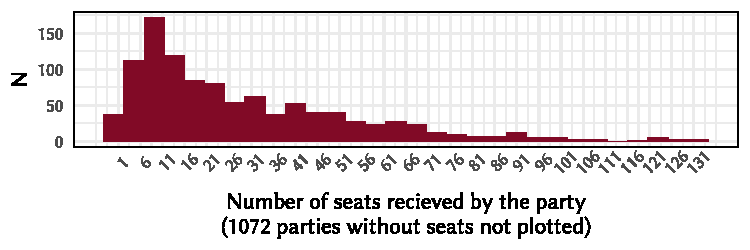
\includegraphics[width = \linewidth]{cbfiles/pscplot.pdf}
\end{minipage}


\end{longtable}

\begin{longtable}{p{3.2cm}| p{11cm}}
\texttt{party\_sshare} &\textbf{Party Seat Share}\newline 
Share of seats recieved by the party.

\hspace*{.25cm}
\begin{minipage}[t]{\linewidth }
\vspace{0pt}
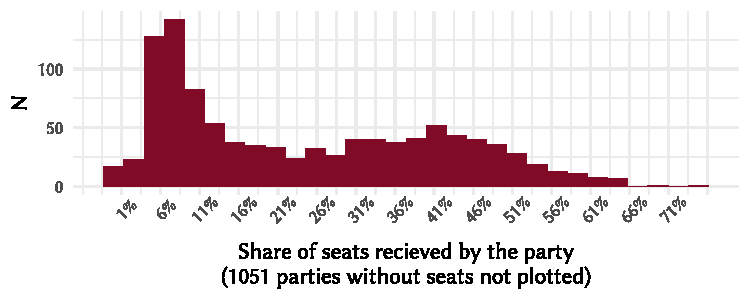
\includegraphics[width = \linewidth]{cbfiles/pssplot.pdf}
\end{minipage}


\end{longtable}

\begin{longtable}{p{3.2cm}| p{11cm}}
\texttt{party\_female\_mps} &\textbf{Number of female MPs from party}\newline 
Number of female MPs elected for the party. Note that for parties not elected to the new Landtag party\_female\_mps always is marked as missing.

\hspace*{.25cm}
\begin{minipage}[t]{\linewidth }
\vspace{0pt}
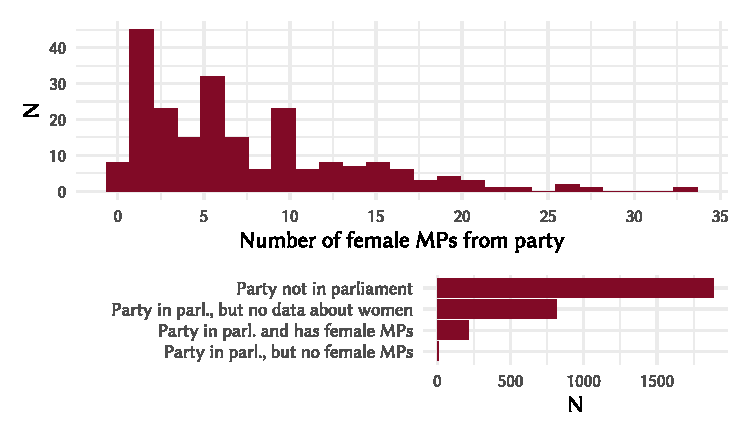
\includegraphics[width = \linewidth]{cbfiles/pfmpcplot.pdf}
\end{minipage}


\end{longtable}

\begin{longtable}{p{3.2cm}| p{11cm}}
\texttt{ppeg\_id} &\textbf{PPEG ID}\newline 
If available, party id of the party in the PPEG database \parencite{ppegDatabasePoliticalParties2022}. These party IDs are chiefly based on party IDs from \textcite{mackieInternationalAlmanacElectoral1991}.


\hspace*{.25cm}
\begin{minipage}[t]{\linewidth }
\vspace{0pt}
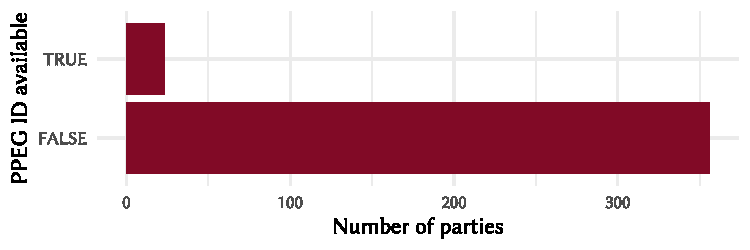
\includegraphics[width = \linewidth]{cbfiles/govelecplot.pdf}
\end{minipage}


\end{longtable}

\begin{longtable}{p{3.2cm}| p{11cm}}
\texttt{ches\_id} &\textbf{CHES ID}\newline 
If available, ID of the party in the Chapel-Hill Expert Survey \parencite{jollyChapelHillExpert2022}.


\hspace*{.25cm}
\begin{minipage}[t]{\linewidth }
\vspace{0pt}
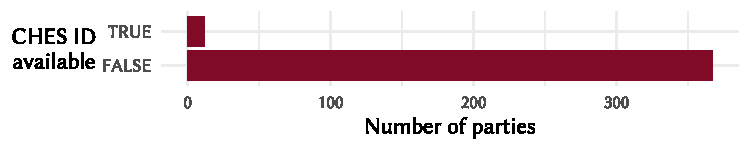
\includegraphics[width = \linewidth]{cbfiles/chesplot.pdf}
\end{minipage}



\end{longtable}

\begin{longtable}{p{3.2cm}| p{11cm}}
\texttt{partyfacts\_id} &\textbf{PartyFacts ID}\newline 
If available, ID of the party in the partyfacts database \parencite{doringPartyFactsDatabase2019}.

\hspace*{.25cm}
\begin{minipage}[t]{\linewidth }
\vspace{0pt}
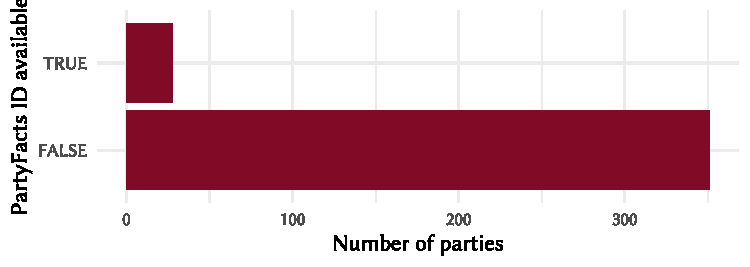
\includegraphics[width = \linewidth]{cbfiles/partyfactsplot.pdf}
\end{minipage}



\end{longtable}

\begin{longtable}{p{3.2cm}| p{11cm}}
\texttt{decker\_neu} &\textbf{Chapter Parteienhandbuch}\newline 
Denotes, wether the Handbuch der deutschen Parteien (3. ed.) by Decker and Neu \parencite{deckerHandbuchDeutschenParteien2018b} has a chapter on the party.

\hspace*{.25cm}
\begin{minipage}[t]{\linewidth }
\vspace{0pt}
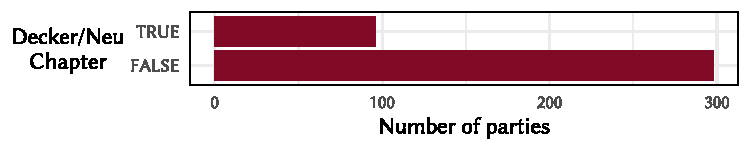
\includegraphics[width = \linewidth]{cbfiles/deckerneuplot.pdf}
\end{minipage}



\end{longtable}

\begin{longtable}{p{3.2cm}| p{11cm}}
\texttt{url\_info} &\textbf{URL with additional info on the party}\newline 
URL to informaton on the party on the web. Can contain multiple URLs!
\end{longtable}

\begin{longtable}{p{3.2cm}| p{11cm}}
\texttt{party\_remarks\_
stelzle} &\textbf{Party remarks Stelzle}\newline 
Remarks on the party by me.
\end{longtable}

\begin{longtable}{p{3.2cm}| p{11cm}}
\texttt{party\_remarks\_
bundeswahlleiter} &\textbf{Party remarks Bundeswahlleiter}\newline 
Remarks on the party as listed by the Bundeswahlleiter.
\end{longtable}

\begin{longtable}{p{3.2cm}| p{11cm}}
\texttt{gueltige\_stimm
-zettel\_hh\_hb} &\textbf{Gültige Stimmzettel HH and HB}\newline 
Messy totals.
\end{longtable}

\begin{longtable}{p{3.2cm}| p{11cm}}
\texttt{gesamtstimmen\_by} &\textbf{Gesamtstimmen BY}\newline 
Messy totals.
\end{longtable}

\begin{longtable}{p{3.2cm}| p{11cm}}
\texttt{ausgefallene\_
stimmen\_be} &\textbf{Ausgefallene Stimmen BE}\newline 
Messy totals.
\end{longtable}

\begin{longtable}{p{3.2cm}| p{11cm}}
\texttt{abgegebene\_
stimmen\_hh} &\textbf{Abgegebene Stimmen HH}\newline 
Messy totals.
\end{longtable}

\begin{longtable}{p{3.2cm}| p{11cm}}
\texttt{ungueltige\_
stimmen\_except\_
hh\_hb} &\textbf{Ungültige Stimmen except in HH and HB}\newline 
Messy totals.
\end{longtable}

\begin{longtable}{p{3.2cm}| p{11cm}}
\texttt{ungueltige\_
stimmzettel\_hh\_hb} &\textbf{Ungültige Stimmzettel in HH and HB}\newline 
Messy totals.
\end{longtable}

\newpage

\hypertarget{ltw_governments}{%
\section{\texorpdfstring{\texttt{ltw\_governments}}{ltw\_governments}}\label{ltw_governments}}

This section of the codebook only concerns variables specific to the
\texttt{ltw\_governments} dataset. For further variables please refer to
the \texttt{ltw\_elections} section.

\texttt{ltw\_governments} is a long-form dataset containing information
on governments in the German states. Each row contains information on
one state government. The data can be accessed in \texttt{R} using
\texttt{bundeslaendeR::ltw\_governments}.

\hypertarget{ltw_governments-variable-information}{%
\subsection{\texorpdfstring{\texttt{ltw\_governments} Variable
Information}{ltw\_governments Variable Information}}\label{ltw_governments-variable-information}}

\begin{longtable}{p{3.2cm}| p{11cm}}
\texttt{gov\_no\_within\_
legterm} &\textbf{Number of cabinet within legislative term}\newline 
Number of cabinet within legislative term (e.g. First/Second/Third/... cabinet in the 1990-1994 legislative term of state X).



\hspace*{.25cm}
\begin{minipage}[t]{\linewidth }
\vspace{0pt}
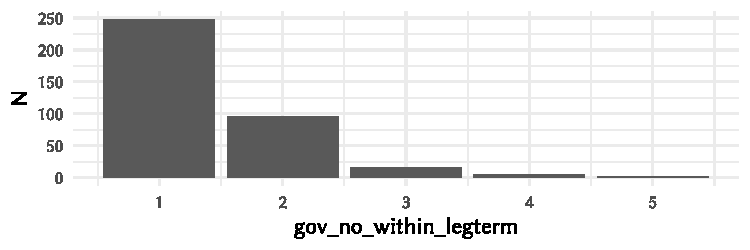
\includegraphics[width = \linewidth]{cbfiles/govnolegperplot.pdf}
\end{minipage}



\end{longtable}

\begin{longtable}{p{3.2cm}| p{11cm}}
\texttt{gov\_id} &\textbf{Government ID}\newline 
Unique ID of government. Taken from Linhart et al. However, this ID is not counting up within state by time. In cases where Governments were 
           missing from Linhart et al. before the timeframe covered by Linhart et al. (eg. in Berlin) these earlyer governments have a higher ID than later cabinets 
           contained in Linhart et al. data.
\end{longtable}

\begin{longtable}{p{3.2cm}| p{11cm}}
\texttt{state\_gov\_number} &\textbf{Number of government in state.}\newline 
Number of government in state.



\hspace*{.25cm}
\begin{minipage}[t]{\linewidth }
\vspace{0pt}
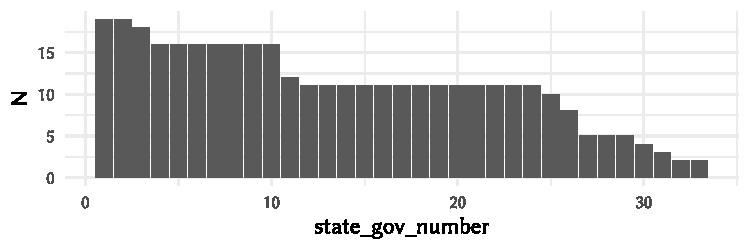
\includegraphics[width = \linewidth]{cbfiles/stategovnumplot.pdf}
\end{minipage}



\end{longtable}

\begin{longtable}{p{3.2cm}| p{11cm}}
\texttt{gov\_start\_date} &\textbf{Government Starting Date}\newline 
Starting date of the government.  ISO 8601 or R-Date format.






\hspace*{.25cm}
\begin{minipage}[t]{\linewidth }
\vspace{0pt}
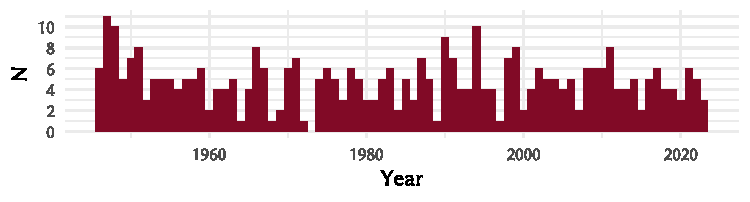
\includegraphics[width = \linewidth]{cbfiles/govstartdatesplot.pdf}
\end{minipage}






\end{longtable}

\begin{longtable}{p{3.2cm}| p{11cm}}
\texttt{gov\_source} &\textbf{Government Source}\newline 
Source of the information on the government. Either Linhart et al. or the URL of the German Wikipedia Page containing information on the cabinet.
\end{longtable}

\begin{longtable}{p{3.2cm}| p{11cm}}
\texttt{gov\_remarks\_
stelzle} &\textbf{Governments remarks Stelzle}\newline 
My remarks on governments.
\end{longtable}

\begin{longtable}{p{3.2cm}| p{11cm}}
\texttt{minister\_president} &\textbf{Name of minister president}\newline 
Name of minister president.
\end{longtable}

\begin{longtable}{p{3.2cm}| p{11cm}}
\texttt{mp\_party} &\textbf{Minister President's Party}\newline 
Party of the minister president. partyname\_short format used. Note: There is a single cabinet with an independent minister president: Heinrich Welsch's caretaker government in the Saarland (at the time not yet a member of the FRG) in 1955. Further note that there is a single case where the party denoted as \texttt{mp\_party} is not part of the set of parties in \texttt{gov\_parties}. Hamburg's mayor Kurt Sieveking (1953-1957) was a member of the CDU and is denoted as such in \texttt{mp\_party}. However, the CDU contested the 1953 Hamburg election as part of the Hamburg-Block electoral alliance together with the FDP, the DP and the BHE. Thus, as there are no separate election results for the member-parties of the electoral alliance available, \texttt{gov\_parties} is here just denoted as \texttt{HamburgBlock/VBH}.
\end{longtable}

\begin{longtable}{p{3.2cm}| p{11cm}}
\texttt{gov\_parties} &\textbf{Names of Government Parties}\newline 
String containing the names (partyname\_short format) of all government parties separated by ' $\sim$ '. The MP's party first, followed by other government parties in the order of their seatshare.
\end{longtable}

\begin{longtable}{p{3.2cm}| p{11cm}}
\texttt{gov\_vshare} &\textbf{Government Vote Share}\newline 
Collective vote share of government parties.

\hspace*{.25cm}
\begin{minipage}[t]{\linewidth }
\vspace{0pt}
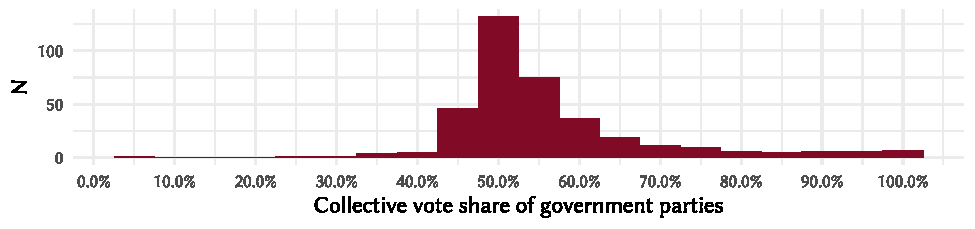
\includegraphics[width = \linewidth]{cbfiles/gvsplot.pdf}
\end{minipage}


\end{longtable}

\begin{longtable}{p{3.2cm}| p{11cm}}
\texttt{gov\_seat\_count} &\textbf{Government Seat Count}\newline 
Collective number of seats of government parties.

\hspace*{.25cm}
\begin{minipage}[t]{\linewidth }
\vspace{0pt}
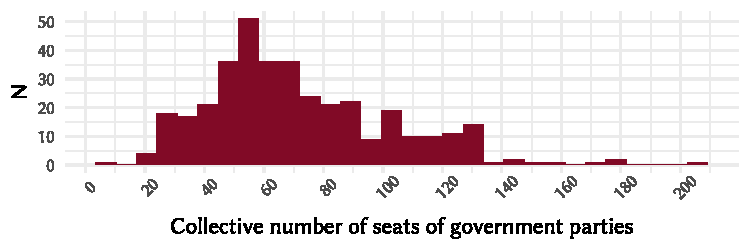
\includegraphics[width = \linewidth]{cbfiles/gscplot.pdf}
\end{minipage}


\end{longtable}

\begin{longtable}{p{3.2cm}| p{11cm}}
\texttt{gov\_sshare} &\textbf{Government Seat Share}\newline 
Share of seats of government parties.

\hspace*{.25cm}
\begin{minipage}[t]{\linewidth }
\vspace{0pt}
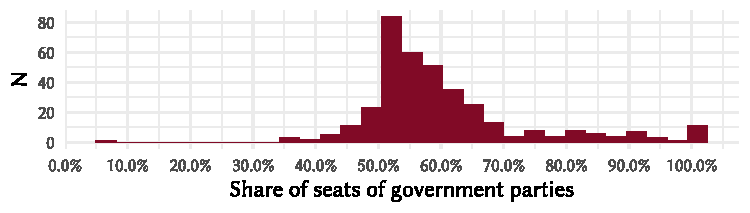
\includegraphics[width = \linewidth]{cbfiles/gssplot.pdf}
\end{minipage}


\end{longtable}

\begin{longtable}{p{3.2cm}| p{11cm}}
\texttt{gov\_tog} &\textbf{Type of Government}\newline 
\begin{flushleft}\vspace{-0.8cm}Type of Government:\setlist{nolistsep}\begin{itemize}[noitemsep]\item Single Party Majority \item Oversized Coalition \item Minimal Winning Coalition \item Single Party Minority \item Multi Party Majority \item Caretaker. \end{itemize}Note that this classification is done automatically based on the number of seats of each governing party \emph{at the beginning of the legislative term}. MPs defecting between parties and thus potentially changing the majority status of governments can thus not be incorporated!
\end{flushleft}
\end{longtable}

\newpage

\hypertarget{ltw_combined}{%
\section{\texorpdfstring{\texttt{ltw\_combined}}{ltw\_combined}}\label{ltw_combined}}

This section of the codebook only concerns variables specific to the
\texttt{ltw\_combined} dataset. For further variables please refer to
the sections on \texttt{ltw\_elections} and \texttt{ltw\_governments}.

\texttt{ltw\_combined} is a long-form dataset containing both election
results as well as linked information on governments in the German
states. Each row contains information on one party during the time in
office of one cabinet. For a schematic version of
\texttt{ltw\_combined}'s structure see table\(~\)\ref{strltwelecgov}.
The data can be accessed in \texttt{R} using
\texttt{bundeslaendeR::ltw\_combined}.

\hypertarget{ltw_combined-variable-information}{%
\subsection{\texorpdfstring{\texttt{ltw\_combined} Variable
Information}{ltw\_combined Variable Information}}\label{ltw_combined-variable-information}}

\begin{longtable}{p{3.2cm}| p{11cm}}
\texttt{gov\_party} &\textbf{Government Party}\newline 
Boolean wether the party was a cabinet party. Note: There is a single cabinet where no party is marked as part of the cabinet: Heinrich Welsch's caretaker government in the Saarland (at the time not yet a member of the FRG) in 1955.
\end{longtable}

\begin{longtable}{p{3.2cm}| p{11cm}}
\texttt{nmin\_party} &\textbf{Number of Ministers of Party}\newline 
Number of ministers of party. Note that the number of party-independent ministers is not collected. Thus, the sum of the number of ministers of all government parties can not reliably be understood as the size of the cabinet.



\hspace*{.25cm}
\begin{minipage}[t]{\linewidth }
\vspace{0pt}
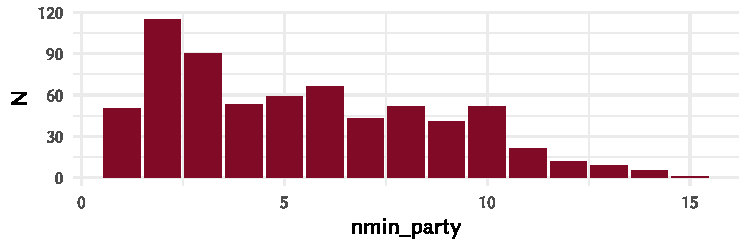
\includegraphics[width = \linewidth]{cbfiles/nminpartyplot.pdf}
\end{minipage}



\end{longtable}

\begin{longtable}{p{3.2cm}| p{11cm}}
\texttt{is\_mp\_party} &\textbf{Is MP Party?}\newline 
Is the governments minister president from this party? Note: There are two cases of cabinets where the minister president is not part of any party contesting the election: 1) Heinrich Welsch's caretaker government in the Saarland (at the time not yet a member of the FRG) in 1955. 2) Hamburg's mayor Kurt Sieveking (1953-1957) was a member of the CDU and is denoted as such in \texttt{mp\_party}. However, the CDU contested the 1953 Hamburg election as part of the Hamburg-Block electoral alliance together with the FDP, the DP and the BHE. Thus, as there are no separate election results for the member-parties of the electoral alliance available and only the election result of the entire electoral alliance is reported, \texttt{is\_mp\_party} is set to \texttt{FALSE} for all parties during the cabinet's tenure, including for the Hamburg-Block.
\end{longtable}

\newpage

\begin{landscape}

    \setcounter{table}{1}
\begin{table}

\normalsize
\caption{Structure of \texttt{ltw\_combined}}
\label{strltwelecgov}
\centering
\tiny
\texttt{
    \begin{tabular}{llrllrllrllrllrllr}
        \toprule
        \multicolumn{3}{c}{\textbf{\textsf{State Variables}}} & \multicolumn{3}{c}{\textbf{\textsf{Election Variables}}} & \multicolumn{3}{c}{\textbf{\textsf{Party Variables}}} & \multicolumn{3}{c}{\textbf{\textsf{Party-Election Variables}}} &
        \multicolumn{3}{c}{\textbf{\textsf{Government Variables}}} &
        \multicolumn{3}{c}{\textbf{\textsf{Government-Party Variables}}} \\
        \multicolumn{3}{c}{\textsf{Name, Abbreviation,}} & \multicolumn{3}{c}{\textsf{Election date, Size}} & \multicolumn{3}{c}{\textsf{Names, Abbreviations, several IDs}} & \multicolumn{3}{c}{\textsf{Vote Count, -Share, Seat}}&
        \multicolumn{3}{c}{\textsf{Inauguration date, PM Name, gov.}} &
        \multicolumn{3}{c}{\textsf{Status in government, number of}}\\
        \multicolumn{3}{c}{\textsf{NUTS1 Code}} &
        \multicolumn{3}{c}{\textsf{Electorate, Turnout, ...}} &
        \multicolumn{3}{c}{\textsf{several IDs}} &
        \multicolumn{3}{c}{\textsf{Count, -Share, ...}} &
        \multicolumn{3}{c}{\textsf{numbering, gov\_id, ...}} &
        \multicolumn{3}{c}{\textsf{party ministers, ...}} \\
        \cmidrule(r){1-3}\cmidrule(lr){4-6}\cmidrule(lr){7-9}
        \cmidrule(lr){10-12}\cmidrule(lr){13-15}\cmidrule(l){16-18}
        \textbf{state} & \textbf{nuts1} & \textbf{...} & \textbf{election\_date} & \textbf{turnout} & \textbf{...} & \textbf{partyname\_short} & \textbf{ches\_id} & \textbf{...} & \textbf{party\_vshare} & \textbf{party\_seat\_count} & \textbf{...} & \textbf{gov\_start\_date} & \textbf{minister\_president} & \textbf{...} & \textbf{gov\_party} & \textbf{nmin\_party} & \textbf{...} \\
        \midrule
        BE & DE3 & ... & 2015-09-18 & 0.765 & ... & Party A & 001 & ... & 0.45 & 46 & ... & 2015-10-07 & Mustermann, Max & ... & TRUE & 7 & ... \\
        BE & DE3 & ... & 2015-09-18 & 0.765 & ... & Party B & 002 & ... & 0.30 & 12 & ... & 2015-10-07 & Mustermann, Max & ... & TRUE & 4 & ... \\
        BE & DE3 & ... & 2015-09-18 & 0.765 & ... & Party C & 003 & ... & 0.25 & 18 & ...& 2015-10-07 & Mustermann, Max & ... & FALSE & NA & ... \\
        &&&&&&&&&&&\\[-2ex]
        BE & DE3 & ... & 2015-09-18 & 0.765 & ... & Party A & 001 & ... & 0.45 & 46 & ... & 2017-02-28 & Mustermann, Max & ... & TRUE & 11 & ... \\
        BE & DE3 & ... & 2015-09-18 & 0.765 & ... & Party B & 002 & ... & 0.30 & 12 & ... & 2017-02-28 & Mustermann, Max & ... & FALSE & NA & ...\\
        BE & DE3 & ... & 2015-09-18 & 0.765 & ... & Party C & 003 & ... & 0.25 & 18 & ... & 2017-02-28 & Mustermann, Max & ... & FALSE & NA & ...\\
        &&&&&&&&&&&\\
        NI & DE9 & ... & 2012-12-16 & 0.560 & ... & Party A & 001 & ... & 0.17 & 12 & ... & 2013-01-07 & Musterfrau, Erika & ... & FALSE & NA & ...\\
        NI & DE9 & ... & 2012-12-16 & 0.560 & ... & Party B & 002 & ... & 0.33 & 27 & ... & 2013-01-07 & Musterfrau, Erika & ... & FALSE & NA & ...\\
        NI & DE9 & ... & 2012-12-16 & 0.560 & ... & Party D & 004 & ... & 0.50 & 46 & ... & 2013-01-07 & Musterfrau, Erika & ... & TRUE & 13 & ...\\
        \bottomrule
\end{tabular}}
\end{table}

\end{landscape}

\newpage

\hypertarget{ltw_elections_meta}{%
\section{\texorpdfstring{\texttt{ltw\_elections\_meta}}{ltw\_elections\_meta}}\label{ltw_elections_meta}}

This section of the codebook only concerns variables specific to the
\texttt{ltw\_elections\_meta} dataset. For further variables please
refer to the sections on \texttt{ltw\_elections}.

\texttt{ltw\_elections\_meta} is a long-format dataset containing meta
information on election results. Each row contains information on one
election. The data can be accessed in \texttt{R} using
\texttt{bundeslaendeR::ltw\_elections\_meta}.

For a discussion of the various measures quantifying party system
properties see \textcite{niedermayerAnalyseParteiensystemen2013}. For
descriptions of the various measures of electoral disproportionality see
\textcite{karpovMeasurementDisproportionalityProportional2008}.

\hypertarget{ltw_elections_meta-variable-information}{%
\subsection{\texorpdfstring{\texttt{ltw\_elections\_meta} Variable
Information}{ltw\_elections\_meta Variable Information}}\label{ltw_elections_meta-variable-information}}

Unless specified otherwise, in the following section \(v_i\) refers to
party \(i\)'s vote share, \(s_i\) to party \(i\)'s seat share and \(n\)
refers to the number of parties contesting a given election.

\begin{longtable}{p{3.2cm}| p{11cm}}
\texttt{number\_parties} &\textbf{Number of parties contesting the election}\newline 
Number of parties $n$ contesting the election.



\hspace*{.25cm}
\begin{minipage}[t]{\linewidth }
\vspace{0pt}
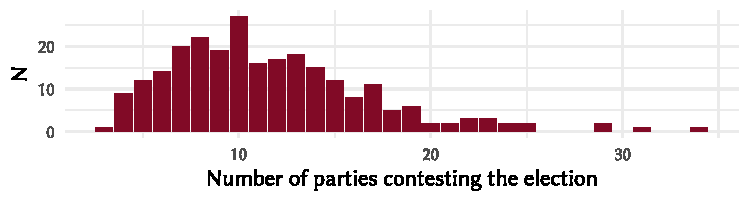
\includegraphics[width = \linewidth]{cbfiles/npartiesplot.pdf}
\end{minipage}



\end{longtable}

\begin{longtable}{p{3.2cm}| p{11cm}}
\texttt{number\_parties\_
parliament} &\textbf{Number of parties gaining seats in the state parliament}\newline 
Number of parties gaining seats in the state parliament.



\hspace*{.25cm}
\begin{minipage}[t]{\linewidth }
\vspace{0pt}
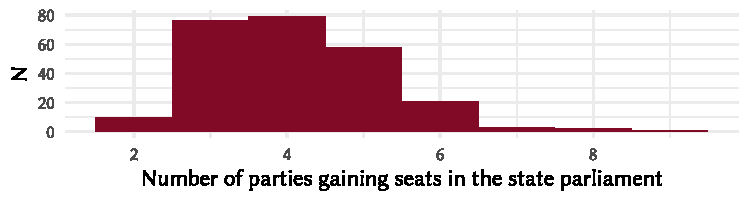
\includegraphics[width = \linewidth]{cbfiles/npartiesparlplot.pdf}
\end{minipage}



\end{longtable}

\begin{longtable}{p{3.2cm}| p{11cm}}
\texttt{fragmentation\_enep} &\textbf{Effective number of parties in the electorate}\newline 
Effective number of parties in the electorate $N_{2 \text{ electorate}}$ \parencite{laaksoEffectiveNumberParties1979}:
           \begin{equation}N_{2 \text{ electorate}} = \frac{1}{\sum_{i = 1}^{n}v_{i}^{2}}. \end{equation}



\hspace*{.25cm}
\begin{minipage}[t]{\linewidth }
\vspace{0pt}
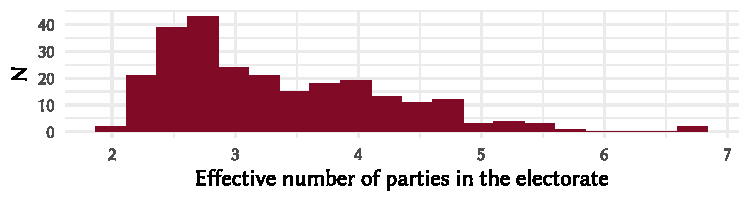
\includegraphics[width = \linewidth]{cbfiles/enepplot.pdf}
\end{minipage}



\end{longtable}

\begin{longtable}{p{3.2cm}| p{11cm}}
\texttt{fragmentation\_enpp} &\textbf{Effective number of parties in parliament}\newline 
Effective number of parties in parliament $N_{2 \text{ parliament}}$ \parencite{laaksoEffectiveNumberParties1979}:
           \begin{equation}N_{2 \text{ parliament}} = \frac{1}{\sum_{i = 1}^{n}s_{i}^{2}}. \end{equation}



\hspace*{.25cm}
\begin{minipage}[t]{\linewidth }
\vspace{0pt}
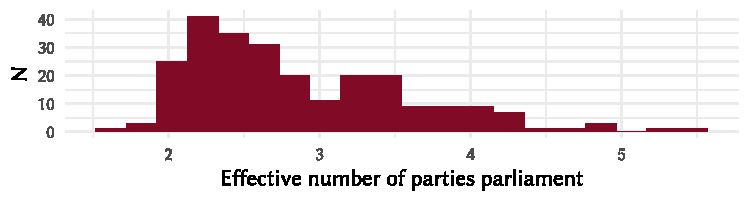
\includegraphics[width = \linewidth]{cbfiles/enppplot.pdf}
\end{minipage}



\end{longtable}

\begin{longtable}{p{3.2cm}| p{11cm}}
\texttt{fragmentation\_rae} &\textbf{Rae's index of fragmentation}\newline 
Rae's index of fragmentation \parencite{raeNoteFractionalizationEuropean1968}:
           \begin{equation}F = 1 - \sum_{i = 1}^{n}v_{i}^{2}.\end{equation}



\hspace*{.25cm}
\begin{minipage}[t]{\linewidth }
\vspace{0pt}
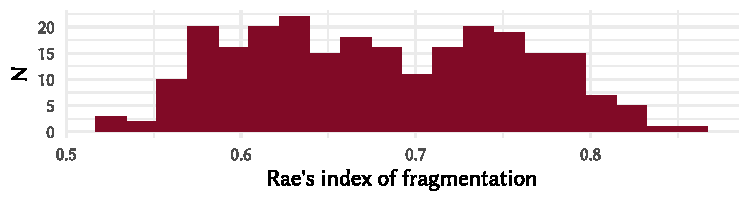
\includegraphics[width = \linewidth]{cbfiles/fragrae.pdf}
\end{minipage}



\end{longtable}

\begin{longtable}{p{3.2cm}| p{11cm}}
\texttt{volatility\_pedersen} &\textbf{Pederson Index of electoral volatility}\newline 
Pederson Index of electoral volatility \parencite{pedersenDynamicsEuropeanParty1979}:
           \begin{equation} V_t = \sum_{i = 1}^{n_t \wedge n_{t-1}}|v_{i,t} - v_{i,t-1}|.  \end{equation} 
           If a party did not contest an election $t$ or $t-1$ it's voteshare for the respective election $v_t$ or $v_{t-1}$ is $0$.
           Attention: These figures probably slightly overestimate the real extent of electoral volatility, as party splits/mergers are not considered: If parties A ($7\%$ at $t-1$) and B ($4\%$ at $t-1$) contest election $t-1$ separately but merge before contesting election $t$ and gaining $15\%$ under the label of party A, they really only contribute $|(7\% + 4\%) - 15\%| = 4\%$ to the calculation of the Pedersen Index. Here, they would contribute $|7\% - 15\%| + |4\% - 0\%| = 12\%$ to the calculation as the merger is not properly accounted for.



\hspace*{.25cm}
\begin{minipage}[t]{\linewidth }
\vspace{0pt}
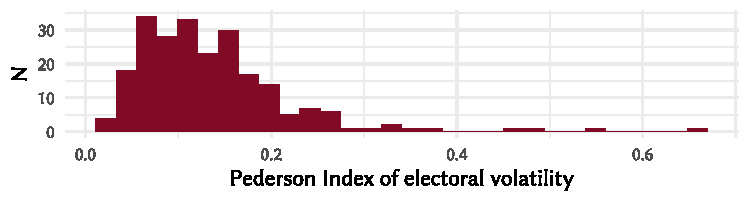
\includegraphics[width = \linewidth]{cbfiles/pedersenplot.pdf}
\end{minipage}



\end{longtable}

All of the disproportionality measures presented here, their calculation
and properties are presented and discussed in
\textcite{karpovMeasurementDisproportionalityProportional2008}. The
distributions of these measures are presented in figure
\ref{fig:distdisp} below.

\begin{longtable}{p{3.2cm}| p{11cm}}
\texttt{disprop\_
max\_deviation} &\textbf{Maximum deviation index of electoral disproportionality}\newline 
Maximum deviation index of electoral disproportionality:
           \begin{equation}MD = \max_{i=\overline{1,n}} |s_i - v_i|.\end{equation}
\end{longtable}

\begin{longtable}{p{3.2cm}| p{11cm}}
\texttt{disprop\_rae} &\textbf{Rae's index of electoral disproportionality}\newline 
Rae's index of electoral disproportionality \parencite{raePoliticalConsequencesElectoral1971}:
           \begin{equation}I_{\text{Rae}} = \frac{1}{n}\sum_{i = 1}^{n}|s_i - v_i|.\end{equation}
\end{longtable}

\begin{longtable}{p{3.2cm}| p{11cm}}
\texttt{disprop\_
loosmore\_hanby} &\textbf{Loosemore-Hanby index of electoral disproportionality}\newline 
Loosemore-Hanby index of electoral disproportionality \parencite{loosemoreTheoreticalLimitsMaximum1971}:
           \begin{equation}I_{\text{LH}} = \frac{1}{2}\sum_{i = 1}^{n}|s_i - v_i|.\end{equation}
\end{longtable}

\begin{longtable}{p{3.2cm}| p{11cm}}
\texttt{disprop\_grofman} &\textbf{Grofman index of electoral disproportionality}\newline 
Grofman index of electoral disproportionality:
           \begin{equation}I_{\text{G}} = \frac{1}{N_{2\text{ electorate}}}\sum_{i=1}^{n}|s_i - v_i|.\end{equation}
\end{longtable}

\begin{longtable}{p{3.2cm}| p{11cm}}
\texttt{disprop\_lijphart} &\textbf{Lijphart index of electoral disproportionality}\newline 
Lijphart index of electoral disproportionality:
           \begin{equation}I_{\text{L}} = \frac{|s_i - v_i| + |s_i - v_i|}{2}\end{equation}
           where only the two largest parties are considered.
\end{longtable}

\begin{longtable}{p{3.2cm}| p{11cm}}
\texttt{disprop\_gallagher} &\textbf{Gallagher index of electoral disproportionality}\newline 
Gallagher index of electoral disproportionality / least squares index (Lsq):
          \begin{equation}Lsq = \sqrt{\frac{1}{2}\sum_{i = 1}^{n}\left(s_i - v_i\right)}.\end{equation}
\end{longtable}

\begin{longtable}{p{3.2cm}| p{11cm}}
\texttt{disprop\_monroe} &\textbf{Monroe index of electoral disproportionality}\newline 
Monroe index of electoral disproportionality:
           \begin{equation}I_{\text{Monroe}} = \sqrt{\frac{\sum_{i=1}^{n}\left(s_i - v_i\right)^2}{1 + \sum_{i=1}^{n}v_i^2}}.\end{equation}
\end{longtable}

\begin{longtable}{p{3.2cm}| p{11cm}}
\texttt{disprop\_gatev} &\textbf{Gatev index of electoral disproportionality}\newline 
Gatev index of electoral disproportionality:
           \begin{equation}I_{\text{Gatev}} = \sqrt{\frac{\sum_{i=1}^{n}\left(s_i - v_i\right)^2}{\sum_{i=1}^{n}\left(s_i^2 + v_i^2\right)}}\end{equation}
\end{longtable}

\begin{longtable}{p{3.2cm}| p{11cm}}
\texttt{disprop\_ryabtsev} &\textbf{Ryabtsev  index of electoral disproportionality}\newline 
Ryabtsev  index of electoral disproportionality:
           \begin{equation}I_{\text{Ryabtsev}} = \sqrt{\frac{\sum_{i=1}^{n}\left(s_i - v_i\right)^2}{\sum_{i=1}^{n}\left(s_i + v_i\right)^2}}.\end{equation}
\end{longtable}

\begin{longtable}{p{3.2cm}| p{11cm}}
\texttt{disprop\_szalai} &\textbf{Szalai index of electoral disproportionality}\newline 
Szalai index of electoral disproportionality:
           \begin{equation}I_{\text{Szalai}} = \sqrt{\frac{\sum_{i=1}^{n}\left(\frac{s_i-v_i}{s_i+v_i}\right)^2}{n}}.\end{equation}
\end{longtable}

\begin{longtable}{p{3.2cm}| p{11cm}}
\texttt{disprop\_
szalai\_weighted} &\textbf{Weighted Szalai index of electoral disproportionality}\newline 
Weighted Szalai index of electoral disproportionality:
           \begin{equation}\tilde{I}_{\text{Szalai}} = \sqrt{\frac{1}{2}\sum_{i=1}^{n}\frac{\left(s_i-v_i\right)^2}{s_i+v_i}}.\end{equation}
\end{longtable}

\begin{longtable}{p{3.2cm}| p{11cm}}
\texttt{disprop\_
aleskerov\_platonov} &\textbf{Aleskerov-Platonov index of electoral disproportionality}\newline 
Aleskerov-Platonov index of electoral disproportionality:
           \begin{equation}R = \frac{1}{k}\sum_{i=1}^{k}\frac{s_i}{v_i}\end{equation}
           where only overrepresented parties are considered.
\end{longtable}

\begin{longtable}{p{3.2cm}| p{11cm}}
\texttt{disprop\_dhondt} &\textbf{D'Hondt index of electoral disproportionality}\newline 
D'Hondt index of electoral disproportionality:
           \begin{equation}H = \max_{i=\overline{1,n}}\frac{s_i}{v_i}.\end{equation}
\end{longtable}

\begin{longtable}{p{3.2cm}| p{11cm}}
\texttt{disprop\_sainte\_lague} &\textbf{Sainte-Lague index of electoral disproportionality}\newline 
Sainte-Lague index of electoral disproportionality:
           \begin{equation}SL = \sum_{i=1}^{n}v_i\left(\frac{s_i}{v_i}-1\right)^2.\end{equation}
\end{longtable}

\begin{figure}

{\centering 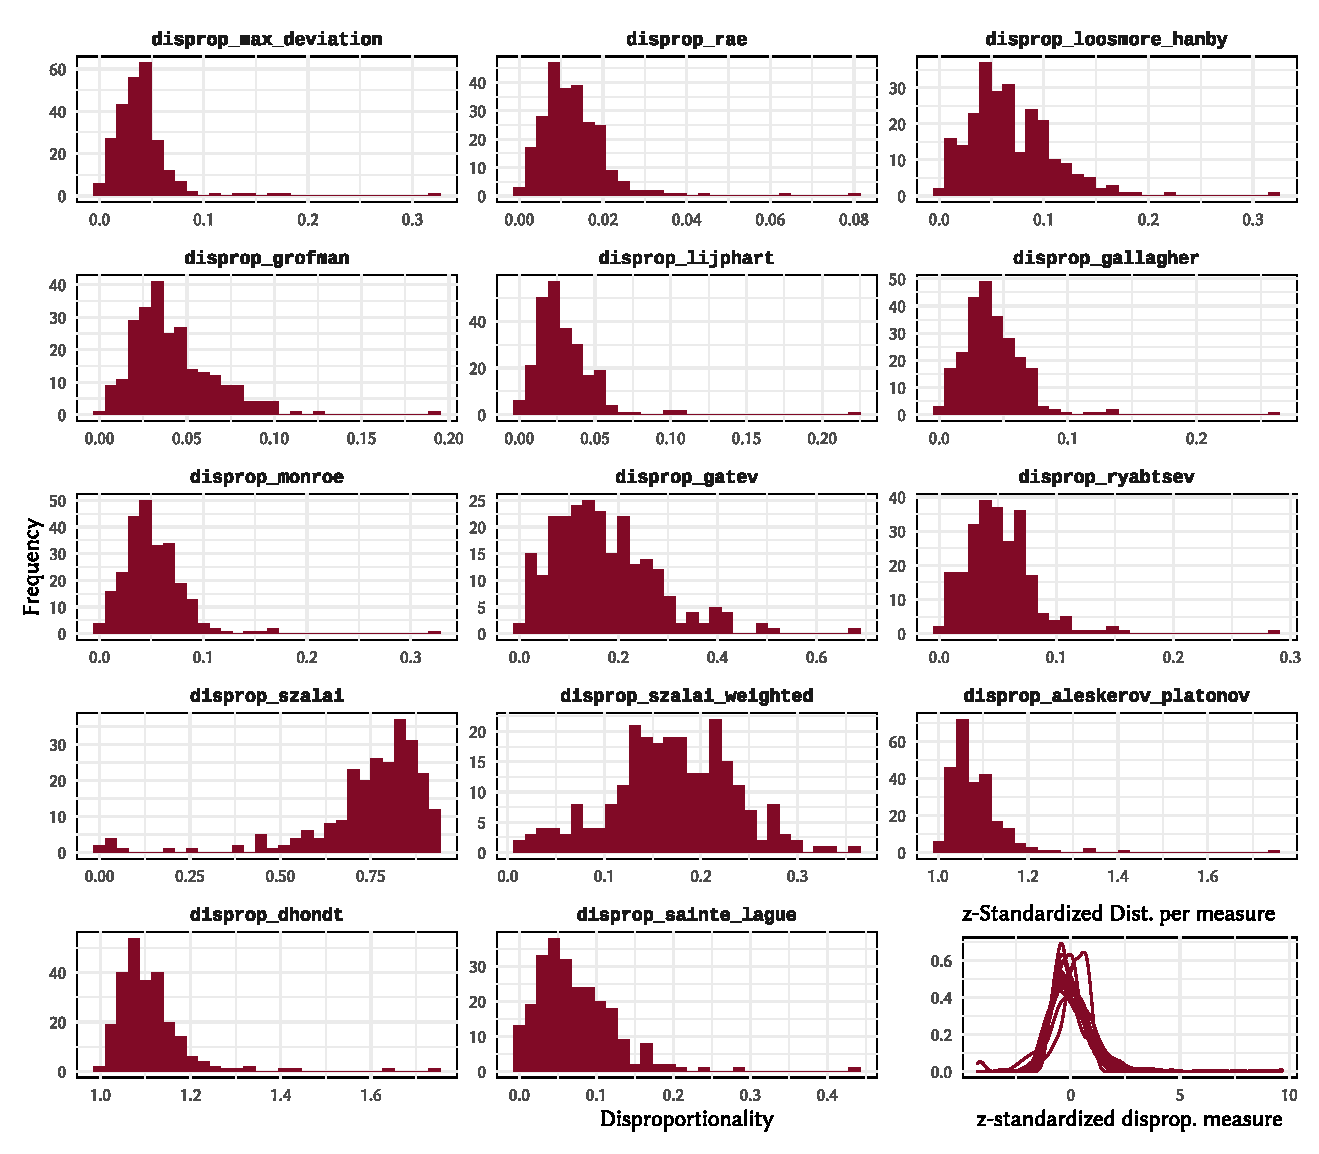
\includegraphics{cbfiles/unnamed-chunk-139-1} 

}

\caption{\label{fig:distdisp}Distribution of Disproportionality Measures}\label{fig:unnamed-chunk-139}
\end{figure}

\clearpage

\hypertarget{link_manifestos-and-link_coalitionagreements}{%
\section{\texorpdfstring{\texttt{link\_manifestos} and
\texttt{link\_coalitionagreements}}{link\_manifestos and link\_coalitionagreements}}\label{link_manifestos-and-link_coalitionagreements}}

\texttt{link\_manifestos} and \texttt{link\_coalitionagreements} provide
easy links of \texttt{bundeslaendeR} data with party manifestos and
coalition agreements made available from polidoc.net - The Political
Documents Archive
\parencites{benoitChallengesEstimatingPolicy2009}{grossDoesEURegional2018}{pappiPolitikpositionenDeutschenLandtagsparteien2014}{pappiPartyElectionProgrammes2009}[for the codebook see][]{brauningerPolidocNetCodebook2018}
and party manifestos from abgeordnetenwatch.de. While file names from
polidoc.net follow a naming pattern
(\texttt{{partyID}.{stateID}.{year}.{1}.{number of party manifesto for election}})
and abgeordnetenwatch.de provides unique IDs through its API, the
provided links make joining the data easier.

Note that polidoc.net provides a manifesto for the Neue Liberale in the
HB 2015 election (41441.005.2015.1.1). Since the party withdrew it's
candidacy before the election and is thus not included in the election
results in \texttt{ltw\_elections}, the manifesto id is not included in
link\_manifestos. Several party manifestos made available through
abgeordnetenwatch.de's API are also not linked, as the respective
parties only contested some nominal districts and not the state-wide
list election and thus no election result is included in
\texttt{ltw\_elections}.

Note that polidoc.net provides a coalition agreement between the SPD and
the Greens following the 2008 HE election (41001.006.2008.1.1). Since
this potential coalition under leadership of SPD politician Andrea
Ypsilanti never came to be due to several SPD MPs opposing the red-green
minority cabinet being externally supported by Die Linke the coalition
agreement can't be matched with a government in \texttt{ltw\_combined}
and is thus not included.

\hypertarget{linking-variables-information}{%
\subsection{Linking-Variables
Information}\label{linking-variables-information}}

The variables \texttt{state}, \texttt{election\_date}, and
\texttt{partyname\_short} can be used in order to link manifestos to the
\texttt{bundeslaendeR} data. How many manifestos are available per
election is plotted in figure\(~\)\ref{figure:manifestoavailability}.

\begin{longtable}{p{3.2cm}| p{11cm}}
\texttt{state} &\textbf{State Abbreviation}\newline 
ISO 3166-2:DE-code of the state.
\end{longtable}

\begin{longtable}{p{3.2cm}| p{11cm}}
\texttt{election\_date} &\textbf{Election Date}\newline 
Date of the election.  ISO 8601 or R-Date format.
\end{longtable}

\begin{longtable}{p{3.2cm}| p{11cm}}
\texttt{partyname\_short} &\textbf{Abbreviated Party Name}\newline 
Harmonized abbreviation of the party's name. 379 unique parties.
\end{longtable}

\begin{longtable}{p{3.2cm}| p{11cm}}
\texttt{polidoc\_filename and polidoc\_filename\_2 in link\_manifestos} &\textbf{Polidoc File Name of Party Manifesto}\newline 
File name of state party manifesto (or 2nd manifesto if available) in \texttt{.txt} format available in The Political Documents Archive (polidoc.net).
\end{longtable}

\begin{longtable}{p{3.2cm}| p{11cm}}
\texttt{agwatch\_pdf\_url in link\_manifestos} &\textbf{URL of Manifesto on \texttt{abgeordnetenwatch.de}}\newline 
URL of the manifesto in \texttt{.pdf} format on \texttt{abgeordnetenwatch.de}.
\end{longtable}

\begin{longtable}{p{3.2cm}| p{11cm}}
\texttt{agwatch\_election\_
manifesto in link\_manifestos} &\textbf{Is an electoral manifesto not just a general manifesto}\newline 
TRUE if the linked manifesto is an electoral manifesto. FALSE if it appears to be a more general manifesto of the party (Grundsatzprogramm) independent of any specific state election.
\end{longtable}

The variable \texttt{gov\_id} can be used in order to link manifestos to
the \texttt{bundeslaendeR} data.

\begin{longtable}{p{3.2cm}| p{11cm}}
\texttt{gov\_id} &\textbf{Government ID}\newline 
Unique ID of government. Taken from Linhart et al. However, this ID is not counting up within state by time. In cases where Governments were 
           missing from Linhart et al. before the timeframe covered by Linhart et al. (eg. in Berlin) these earlyer governments have a higher ID than later cabinets 
           contained in Linhart et al. data.
\end{longtable}

\begin{longtable}{p{3.2cm}| p{11cm}}
\texttt{polidoc\_filename in link\_
coalitionagreements} &\textbf{Polidoc File Name of Coalition Agreement}\newline 
File name of coalition agreement available in The Political Documents Archive (polidoc.net).


\hspace*{.25cm}
\begin{minipage}[t]{\linewidth }
\vspace{0pt}
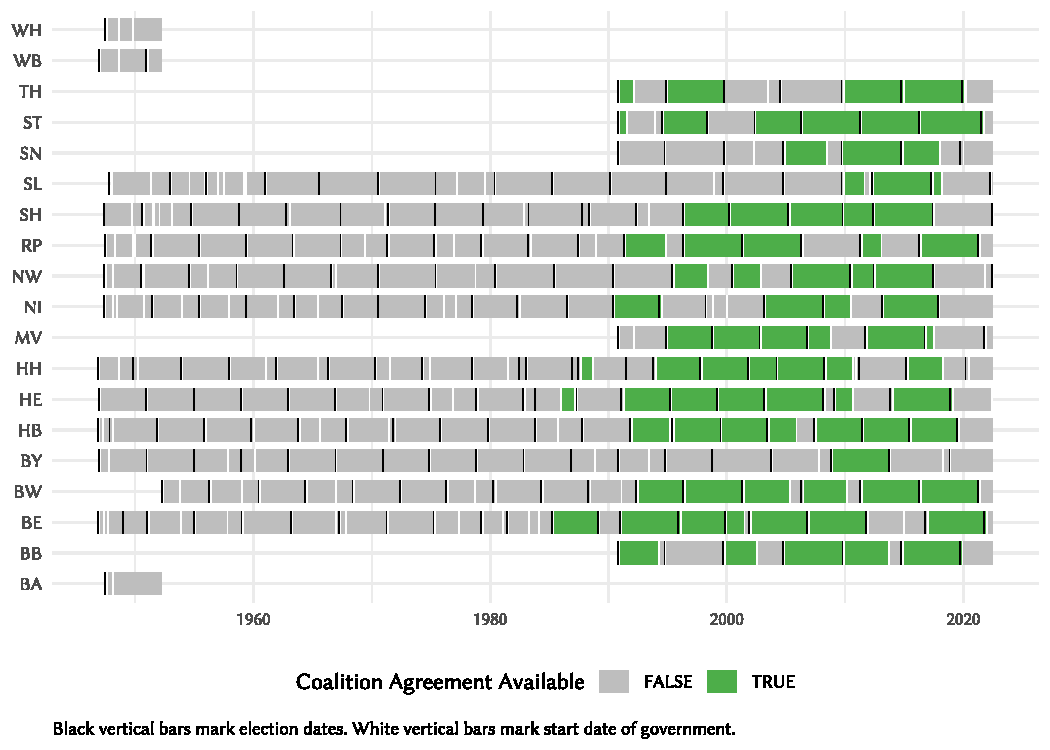
\includegraphics[width = \linewidth]{cbfiles/pltpolidocgov.pdf}
\end{minipage}





\end{longtable}

\newpage

\begin{landscape}

\begin{figure}

{\centering 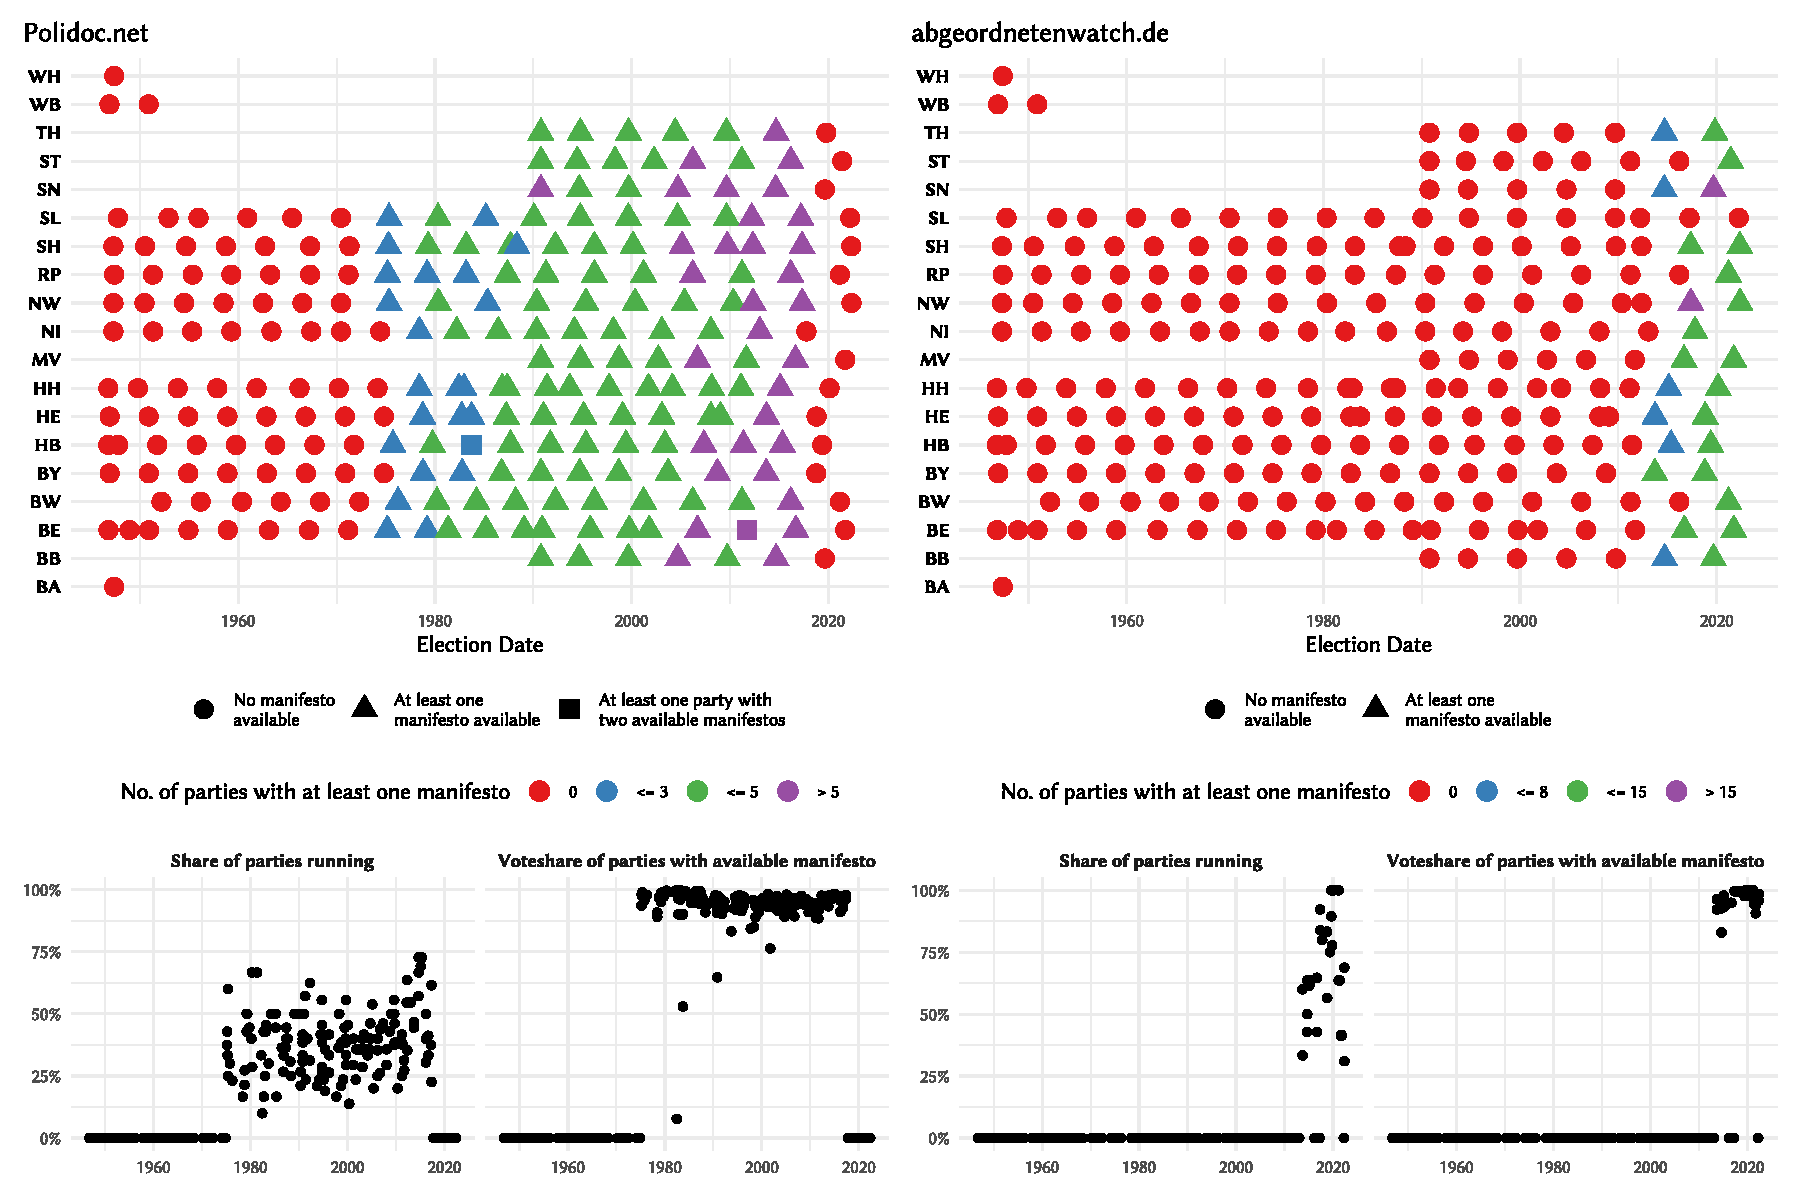
\includegraphics{cbfiles/printmanifestoplot-1} 

}

\caption{\label{figure:manifestoavailability}Availability of manifestos from polidoc.net and abgeordnetenwatch.de}\label{fig:printmanifestoplot}
\end{figure}

\end{landscape}

\newpage

\hypertarget{de_states_grid_4x4}{%
\section{\texorpdfstring{\texttt{de\_states\_grid\_4x4()}}{de\_states\_grid\_4x4()}}\label{de_states_grid_4x4}}

\texttt{de\_states\_grid\_4x4()} exports a data frame containing state
IDs, German and English state names and approximate state locations on a
4x4 grid. The exported data frame can be used to approximately plot
state-facets in their approximate locations using the \texttt{ggplot2}
extension \texttt{geofacet} \autocite{hafenGeofacetGgplot2Faceting2020}.

Please find a comparison of state locations and the grid layout as well
as some example code below.

\hypertarget{example-code}{%
\subsubsection{Example Code:}\label{example-code}}

\begin{Shaded}
\begin{Highlighting}[]
\FunctionTok{library}\NormalTok{(bundeslaendeR)}
\FunctionTok{library}\NormalTok{(tidyverse)}
\FunctionTok{library}\NormalTok{(geofacet)}

\NormalTok{turnout\_plot }\OtherTok{\textless{}{-}}
\NormalTok{ltw\_elections }\SpecialCharTok{\%\textgreater{}\%} 
  \FunctionTok{select}\NormalTok{(state, election\_date, turnout) }\SpecialCharTok{\%\textgreater{}\%} 
  \FunctionTok{distinct}\NormalTok{() }\SpecialCharTok{\%\textgreater{}\%} 
  \FunctionTok{filter}\NormalTok{(}\SpecialCharTok{!}\NormalTok{(state }\SpecialCharTok{\%in\%} \FunctionTok{c}\NormalTok{(}\StringTok{"WB"}\NormalTok{, }\StringTok{"BA"}\NormalTok{, }\StringTok{"WH"}\NormalTok{))) }\SpecialCharTok{\%\textgreater{}\%} 
  \FunctionTok{filter}\NormalTok{(}\SpecialCharTok{!}\FunctionTok{is.na}\NormalTok{(turnout)) }\SpecialCharTok{\%\textgreater{}\%} 
  \FunctionTok{ggplot}\NormalTok{(}\FunctionTok{aes}\NormalTok{(}\AttributeTok{x =}\NormalTok{ election\_date, }\AttributeTok{y =}\NormalTok{ turnout)) }\SpecialCharTok{+}
    \FunctionTok{geom\_line}\NormalTok{(}\AttributeTok{col =} \StringTok{"\#810a26"}\NormalTok{, }\AttributeTok{size =} \FloatTok{1.2}\NormalTok{) }\SpecialCharTok{+}
    \FunctionTok{facet\_geo}\NormalTok{(}\AttributeTok{grid =} \FunctionTok{de\_states\_geofacet\_grid\_4x4}\NormalTok{(}\AttributeTok{linebreak =}\NormalTok{ T),}
              \AttributeTok{facets =} \SpecialCharTok{\textasciitilde{}}\NormalTok{state, }\AttributeTok{label =} \StringTok{"name"}\NormalTok{) }\SpecialCharTok{+}
    \FunctionTok{scale\_y\_continuous}\NormalTok{(}\AttributeTok{limits =} \FunctionTok{c}\NormalTok{(}\DecValTok{0}\NormalTok{,}\DecValTok{1}\NormalTok{),}
                       \AttributeTok{labels =}\NormalTok{ scales}\SpecialCharTok{::}\NormalTok{percent) }\SpecialCharTok{+}
    \FunctionTok{theme}\NormalTok{(}\AttributeTok{strip.text =} \FunctionTok{element\_text}\NormalTok{(}\AttributeTok{face =} \StringTok{"bold"}\NormalTok{)) }\SpecialCharTok{+}
    \FunctionTok{labs}\NormalTok{(}\AttributeTok{x =} \ConstantTok{NULL}\NormalTok{, }\AttributeTok{y =} \StringTok{"Turnout"}\NormalTok{)}
\end{Highlighting}
\end{Shaded}

\nocite{runfolaGeoBoundariesGlobalDatabase2020}

\newpage

\begin{landscape}

\begin{figure}

{\centering 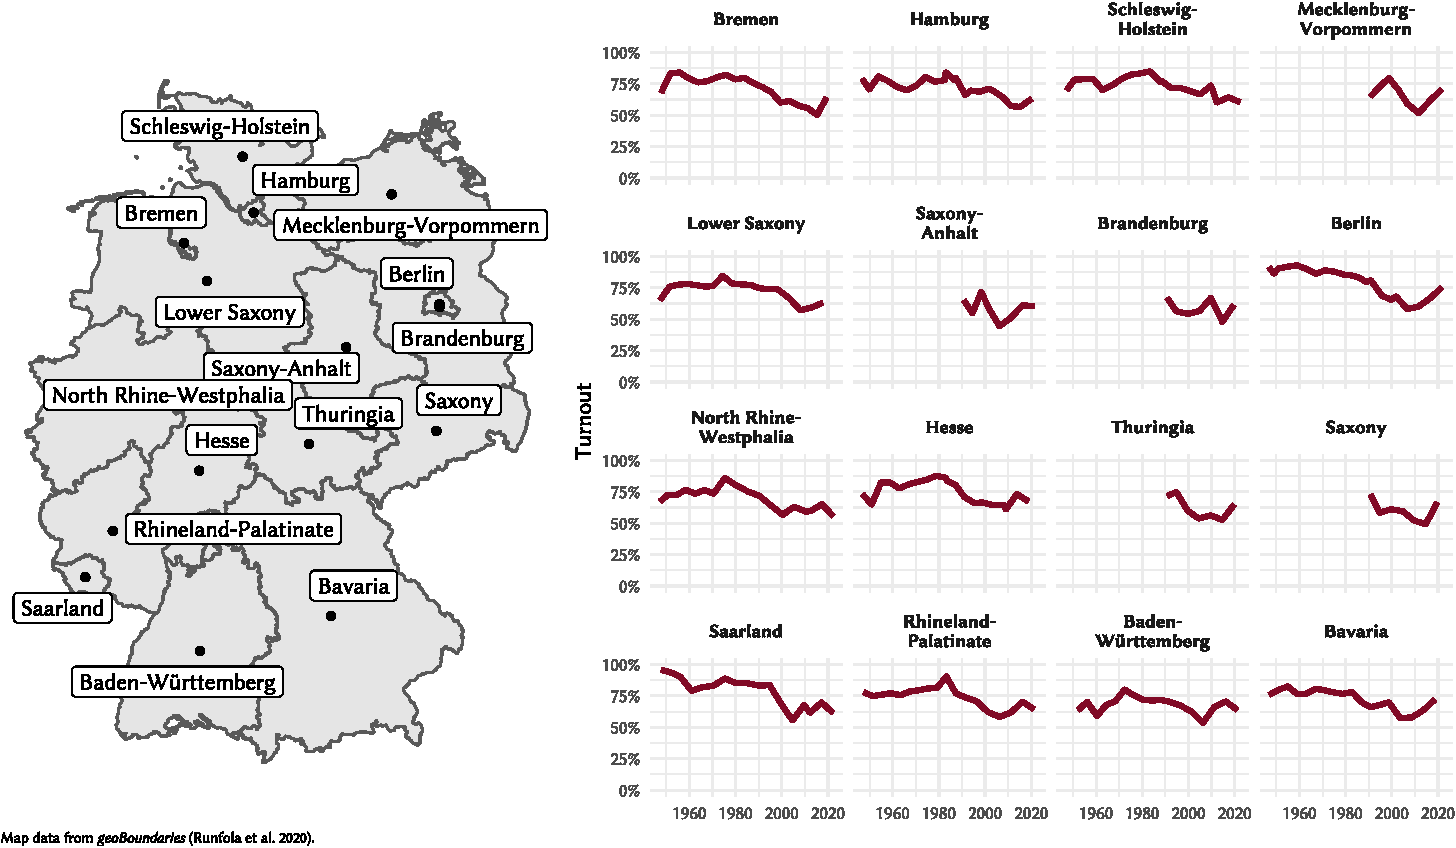
\includegraphics{cbfiles/map-vs-grid-plot-1} 

}

\caption{Comparison of state location and grid layout}\label{fig:map-vs-grid-plot}
\end{figure}

\end{landscape}

\printbibliography[title=References]

\end{document}
